\section{Model development}
We start the simulation with all the atoms on a face-centered cubic lattice, since this corresponds to the crystalline structure of Argon. See figure \ref{face_lattice}.
To build this kind of lattice we need four base-vectors, and several base-position. Let the base position be one of the corners in the lattice-unit. When we have determined the base position $\bf r_{base}$ we can build the 
unit with the four base-vectors.

\begin{align}
 {\bf r_0} = \left[0,0,0\right]\nonumber \\
 {\bf r_{xy}} = \left[\frac{b}{2}, \frac{b}{2}, 0\right]\nonumber \\
 {\bf r_{yz}} = \left[0, \frac{b}{2}, \frac{b}{2}\right]\nonumber \\
 {\bf r_{zx}} = \left[\frac{b}{2}, 0, \frac{b}{2}\right]\nonumber \\
\end{align}
\begin{figure}[H]
 \centering
 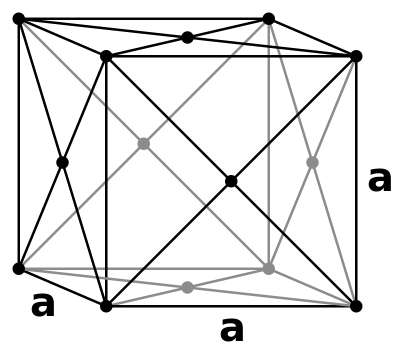
\includegraphics[width=9 cm]{./figures/face_lattice.png}
 % face_lattice.png: 399x351 pixel, 72dpi, 14.08x12.38 cm, bb=0 0 399 351
 \caption{A face-centered cubic lattice unit.}
 \label{face_lattice}
\end{figure}
where $b$ is the distance between the base positions. For solid Argon  $b=5.260 Å$ To make this lattice you first make a grid consisting of the base positions (this is like a three dimensional cartesian coordinate-system, a system made of primitive cubic lattices) and
for each of the base positions you generate four positions:
\begin{align}
&{\bf r_{base} + r_0}\nonumber \\ 
&{\bf r_{base} + r_1}\nonumber \\ 
&{\bf r_{base} + r_2}\nonumber \\ 
&{\bf r_{base} + r_3} \nonumber. \\
\end{align}
The natural choice of datastructure is an atom-class and a lattice class.  The atoms has three aramdillo vectors; position, velocity, force (that works on the atom), and a string that states the type of element (Ar for argon). The Lattice-calls
holds information about the lattice size, the size $b$, temperature and mass. It also holds a vector made of all the atoms in the system. (This is the brute force way of making the system).\\
To visualize the system we make state files; text files with .xyz format. The lines in the state file gives the type element, the position and the velocity of a atom at a given time. These state files can be loaded into VMD or OVITO.
\subsection{Visualization}
Visualization of the lattice made of $N_c \times N_c \times N_c$ face-centered cubic lattice units. This means we have a system of $N_c^3*4$ atoms. See figure \ref{a}.
\begin{figure}[H]
 \centering
 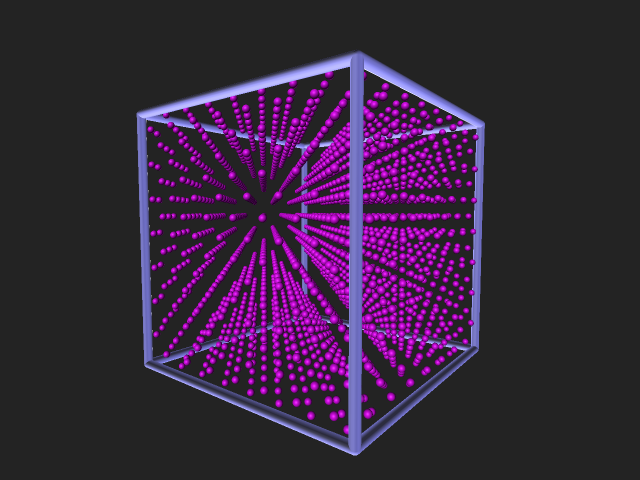
\includegraphics[width=9 cm]{./figures/exerciseA.png}
 % exerciseA.png: 640x480 pixel, 96dpi, 16.93x12.70 cm, bb=0 0 480 360
 \caption{Visualization of solid Argon}
 \label{a}
\end{figure}
To visualize the time development of the system, you make a .xyz file for each timestep and use VMD or OVITO to make an animation from these files.
\subsection{Motion}
We use the Verlet algorithm to find the time development of the system. The velocity and position of each particle is calculated as follows.
\begin{align}
 {\bf v}_i(t + \Delta t/2) &= {\bf v}_i + \frac{{\bf F}_i(t)}{2m}\Delta t\\
 {\bf r}_i(t + \Delta t) &= {\bf r}_i(t) + {\bf v}_i(t + \Delta t/2)\Delta t\\
 {\bf F}_i(t + \Delta t) &= -\nabla_i U_i{\bf r}(t+\Delta t))\\
 {\bf v}_i(t + \Delta t) &= {\bf v}_i(t+ \Delta t/2) + \frac{{\bf F}_i(t+\Delta t}{2m}\Delta t
\end{align}
where we use the Lennard-Jones potential for the interatomic interactions. 
\begin{align}
 U(r) = 4\epsilon\left[ \left(\frac{\sigma}{r}\right)^{12} - \left(\frac{\sigma}{r}\right)^6\right]
\end{align}
where r is the distance between the interacting atoms. We need to calculate the force on each atom due to interactions with all the other atoms in the lattice. Let's find the force on one of the atoms from all the other atoms.
\begin{align}
{\bf F}_i(t) = \sum_{j\neq i} - \nabla_i U_i(|r_j(t)-r_i(t)|)) = \sum_{j\neq i} -24\epsilon \left(\frac{\sigma^6}{r^8} - \frac{2\sigma^{12}}{r^{14}}\right){\bf r} 
\end{align}
where ${\bf r}$ is the vector between the two positions from $r_i$ to $r_j$, and $r$ is the distance between them. The Verlet algorithm: First you have to find the forces on all the atoms at the initial state. Using the force and the velocities, we calculate
the new position of the atoms. Then we have to calculate the force once more, this time using the new positions (the positions at time step $t + \Delta t$ that we just calculated). This force is used to find the velocities at the next time step. And we're done!
The Lennard-Jones potential is plottet in figure \ref{LJ}. To plot this I used $\epsilon = \sigma = 1$, but that is not important. 
\begin{figure}[H]
 \centering
 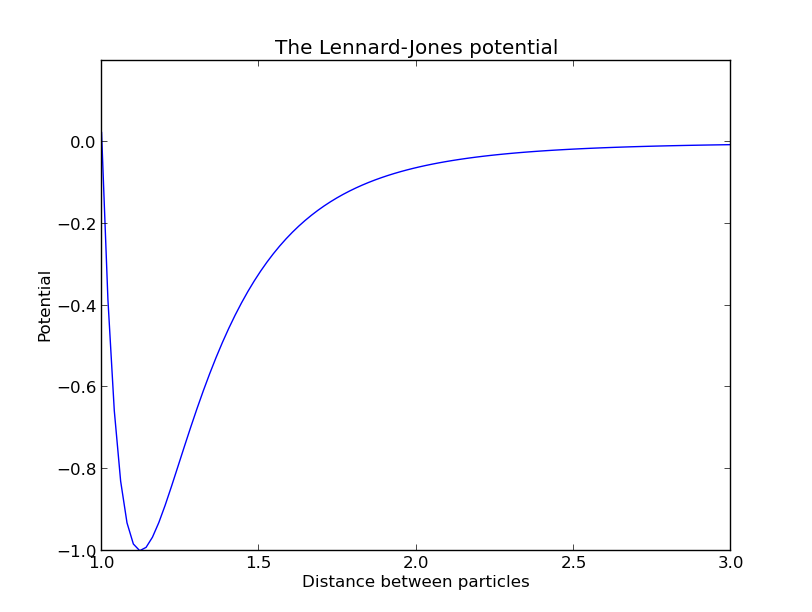
\includegraphics[width=9 cm]{./figures/Lennard_Jones.png}
 % exerciseA.png: 640x480 pixel, 96dpi, 16.93x12.70 cm, bb=0 0 480 360
 \caption{The Lennard-Jones potential}
 \label{LJ}
\end{figure}

From the figure we see that the potential has an extremal point where it has a minimum. This minimum is at a
distance we call equilibrium interatomic distance. When the particles are in a solid state, they will be oscillating with this distance between them. We can find this distance by setting the force between two particles to be zero, and solve for the distance between them.
\begin{align}
 -24\epsilon \left(\frac{\sigma^6}{r^8} - \frac{2\sigma^{12}}{r^{14}}\right){\bf r} &= 0\\
\left(\frac{\sigma^6}{r^8} - \frac{2\sigma^{12}}{r^{14}}\right) & = 0\\
r^6 = 2 \sigma^6\\
r = 1.1225*\sigma.
\end{align}
for Argon, the optimal value of $\sigma = 3.405$Å. The equilibrium interatomic distance is then $r = 3.822$ Å. 

\subsubsection{Periodic boundary conditions}
For our boundaries we choose periodic boundary conditions. This means that if a particle moves out of the cube on one side, it reappears inside the cube on the opposite side of where it disappeard, with the same velocity. We can think about
it as a system of infinity identical cubes lying next to each other (they are copies). So when a particle moves out of the box, so does the copy-particle in the neighbors box. So our box gets a visit from the neightbors copy-particle.
When we calculate the forces we need the distances between the particles. They are calculated using the minimum image convention. 
\begin{figure}
 \centering
 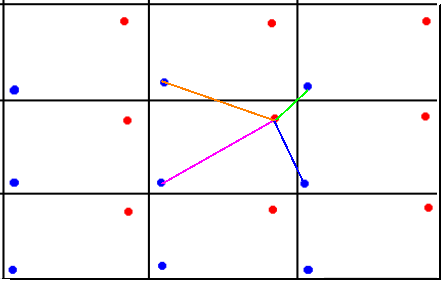
\includegraphics{./figures/periodic.png}
 % exerciseA.png: 640x480 pixel, 96dpi, 16.93x12.70 cm, bb=0 0 480 360
 \caption{The system with periodic boundary conditions. Here with two particles. The lines indicate the choices we have when calculating the distance between the red and the blue particle.}
 \label{periodic}
\end{figure}

Look at figure \ref{periodic}. This drawing illustrates the periodic boundary conditions. The lines in the drawing indicate the choices we have when finding the distance between the two particles. The minimum image convention states that we
choose the smallest distance, in this case; the green line. This limits the interaction range to half the system size.\\
This is done by a set of complicated expressions in my program, but the bottom line is that I find the ``real'' distance $|r_i^x -r_j^x|$ in the x-direction, and the two other options: $|r_i^x - r_j^x \pm L|$, and use the smallest of these three lengths. 
Obviously I do the same evaluation for the y-, and z-direction as well. 

\subsubsection{MD-units}
When doing computations on a computer it is not wise to use very large and very small numbers. Therefore we compute with dimensionless variables, using MD-units. For each variable A in our equtions of motion, we insert $A = A'A_0$, where $A'$
is the variable we end up computing with and $A_0$ is a conversion factor. The time step must also be treated this way. The equation of motion with MD-unit (after finding the equations with MD-units I switched back to variable-names without the aposthrophe. $A'\rightarrow A$.)
\begin{align}
 {\bf v}_i(t + \Delta t/2) &= {\bf v}_i + \frac{{\bf F}_i(t)}{2}\Delta t\nonumber\\
 {\bf r}_i(t + \Delta t) &= {\bf r}_i(t) + {\bf v}_i(t + \Delta t/2)\Delta t\nonumber\\
 {\bf F}_i(t + \Delta t) &= -\nabla_i U_i{\bf r}(t+\Delta t))\nonumber\\
 {\bf v}_i(t + \Delta t) &= {\bf v}_i(t+ \Delta t/2) + \frac{{\bf F}_i(t+\Delta t}{2}\Delta t\nonumber\\
 U(r) &= 4\left[\frac{1}{r^{12}} + \frac{1}{r^6}\right]\nonumber\\
 \sigma_v &= \sqrt{T'}
\end{align}

\subsubsection{Initial velocity}
For the intial velocity we draw random values from a normal distribution with average zero and standard deviation $\sqrt(k_B T/m)$ for each of the components. m is the mass of an atom, and $k_B$ is the Boltzmann constant. Figure \ref{initial_velo} shows the velocities 
before the first time step. The velocities are given in MD-units. For MD-units the standar deviation is $\sigma_v = \sqrt{T'} = \sqrt{T/T0} = 0.914$. This fits quite good with the histogram in figure \ref{initial_velo}.

\begin{figure}[H]
 \centering
 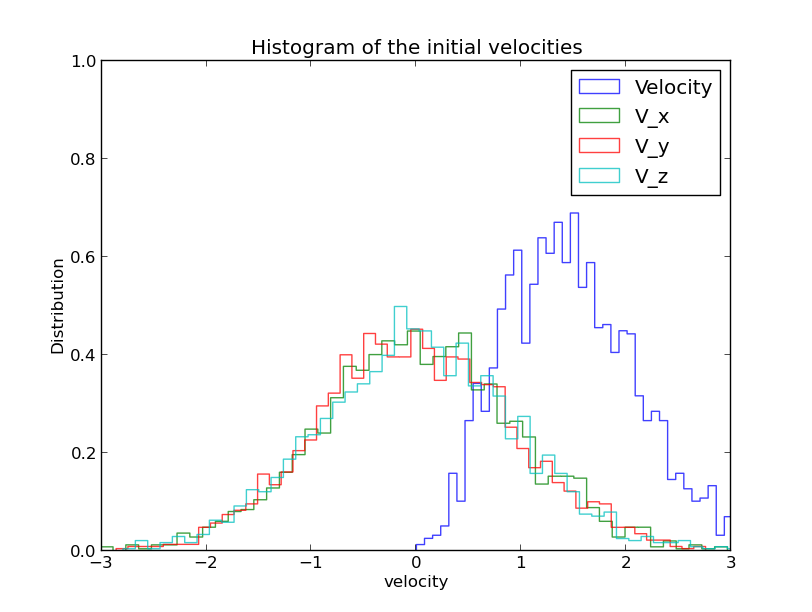
\includegraphics[width=12 cm]{./figures/initial_velo.png}
 % exerciseA.png: 640x480 pixel, 96dpi, 16.93x12.70 cm, bb=0 0 480 360
 \caption{A histogram over the intital velocities of the system. Here in MD-units.}
 \label{initial_velo}
\end{figure}
\subsection{Implementation - Verlet solver}
I ran my program for $8\times 8 \times 8$- lattice, with initial-temperature at 100 K (without thermostat), for 1000 timesteps. The result can be viewed in the gif called movie\_Verlet.gif. 500 timesteps -> 121 s\\
For $8\times 8\times 8$-lattice:\\
\begin{tabular}{|l| c| r|}
\hline
\text{\# time steps}&\text{Verlet Solver-tid(s)} &\text{CellSolver-tid(s)}\\
\hline
 100&24&25 \\
 500&120&123\\
 1000&241&245\\
 \hline
\end{tabular}\\
For $12\times 12\times12$-lattice:\\
\begin{tabular}{|l |c |r|}
\hline
\text{\# time steps}&\text{Verlet Solver-tid(s)} &\text{CellSolver-tid(s)}\\
\hline
 100&274&182 \\
 500&895\text{ (15 min)} &1356\text{( 22 min)}\\
 \hline
\end{tabular}\\

\subsection{Neighbour lists}
The Lennard- Jones interactions is short ranged, and can be neglected for distances over $r_{cut} = 3\L0$. There is not much point in calculating the forces outside this range. We therefore divide the space into quadratic cells of size $r_{cut}$, and let the 
atoms only interact with the atoms in the neighboring cells (and their own cell).
\subsection{Implementation - Neighbour lists}
I ran my program for $8\times 8 \times 8$- lattice, with initial-temperature at 100 K (without thermostat), for 1000 timesteps. The result can be viewed in the gif with the name movie\_cell.gif.  

\subsection{The central limit theorem}
According to the central limit theorem, the velocity distribution of the particles will eventually evolve into a Maxwell-Boltzmann distribution independent of the initial conditions. We test this by starting a simulation with velocities that are uniforml distributed
random numbers in a interval. I made histograms of the x-compontents of the velocities at every time step, and put them together to make a animation. This can be found in movie\_velocity.gif. Here we see that the x components are uniformly distributed at first, but turn into the typical shape of a normal distribution. This happens for 
the y- and z- components as well. When you have a normal distribution for the three space components, the magnitude of the velocity will become a Maxwell-Boltzmann-distribution.  